\documentclass[11pt]{article} 

\usepackage{geometry}
\usepackage[latin1]{inputenc}
\usepackage{cite}
\usepackage{graphicx}
\usepackage{subfig}
\usepackage{times}
\usepackage{setspace}

\newcommand{\fig}[4][htbp]{
  \begin{figure}[#1] {\centering\scalebox{#2}{\includegraphics{fig/#3}}\par}
    \caption{#4\label{#3}}
  \end{figure}
}

\newcommand{\figR}[5][htbp]{
  \begin{figure}[#1]{\centering\scalebox{#2}{\includegraphics[angle=#5]{fig/#3}}\par}
    \caption{#4\label{#3}}
  \end{figure}
}

\newcommand{\figTC}[4][htbp]{
  \begin{figure*}[#1] {\centering\scalebox{#2}{\includegraphics{fig/#3}}\par}
    \caption{#4\label{#3}}
  \end{figure*}
}

\newcommand{\tab}[3][ht]{
  \begin{table}
    \caption{#3}
    \label{#2}
    \centering
    \include{tab/#2}
  \end{table}
}

\newcommand{\hyra}{\textsc{HyRA}}

\newcommand{\hyrafull}{Hybrid Radio Architecture}
%Your submission is limited to twenty two (22) 8.5"x11" double spaced single column pages, using 11pt or larger font. The paper must have one inch margins on both sides, top and bottom The page limit includes everything: references, title, figures, appendices, abstract, etc. Submissions not adhering to these submission guidelines may be rejected by the program chair without further review. Your paper must print satisfactorily on both 8.5"x11" paper and A4 paper: The box containing the text should be no larger than 6.5"x9" (16.5cm x 22.9cm). dfgdfg

\doublespacing

\geometry{papersize={8.5in,11in}, top=1in, bottom=1in, left=1in, right=1in}
%total={6.5in,9in}, 


% Remove the author and date fields and the space associated with them
% from the definition of maketitle!
\makeatletter
\renewcommand{\@maketitle}{
\newpage
 \null
 \vskip 2em%
 \begin{center}%
  {\LARGE \@title \par}%
 \end{center}%
 \par} \makeatother

\begin{document}

\title{A Software-defined Radio Architecture for Embedded Systems}

\author{Tiago Rog�rio M�ck\\ 
\and Roberto de Matos\\ 
\and Ant�nio Augusto Fr�hlich\\  
\and \\
Federal University of Santa Catarina (UFSC)\\
Software/Hardware Integration Lab (LISHA)\\
\{tiago, roberto, guto\}@lisha.ufsc.br\\
}


\maketitle

\begin{abstract}
 Traditional Software-defined Radio architectures cannot go with the
 requirements of embedded systems, specially in terms of performance
 and power consumption. Low-power FPGAs now reaching the market might
 soon become a viable alternative to overcome such limitations. The
 \emph{Hybrid Radio Architecture}~(\hyra) introduced in this paper
 contributes to this scenario as it explores the \emph{Hybrid HW/SW
   Component} concept to enable the implementation of SDRs as direct
 mappings of high-level SDF models.  Although addressing SDR from a
 higher level of abstraction, \hyra\ mechanisms proved far more
 efficient than those behind GNU Radio when the target is a embedded
 reconfigurable hardware platform.
\end{abstract}


%%%%%%%%%%%%%%%%%%%%%%%%%%%%%%%%%%%%%%%%%%%%%%%%%%%%%%%%%%%%%%%%%%%%%%%%%%%%%%
\section{Introduction}
\label{INTRO}

Wireless communication devices are at the heart of a growing number of
embedded systems. Some of them, such as smartphones, must implement
multiple communication protocols (e.g. GSM, GPRS, UMTS, Wi-Fi,
Bluetooth) in face of constantly evolving standards. Others, such as
wireless sensor network gateways, must simultaneously communicate under
multiple protocols and sometimes even dynamically adapt themselves to
preserve connectivity. In this scenario, \emph{Software-defined
  Radio}~(SDR) becomes an appealing approach, since most of the key
components in the communication system---including the physical
layer---are pushed into software, thus making them easy to
reconfigure~\cite{buracchini00}.

However, the implementation of a wireless communication system based
only on an RF front-end, A/D converters, and a processor as illustrated
in figure~\ref{fig_real_sdr2} comes at a high cost.  The associated
\emph{Digital Signal Processing}~(DSP) algorithms demand very high
processing power, a requirement that contradicts major design premises
in the field, which usually include low cost, low energy consumption,
and small size. Nevertheless, it is important to notice that this
exceeding demand for processing power arises basically from the
serialization of essentially parallel algorithms that takes place as
they are pushed from hardware to software, and from the high-latency
datapath typical of software-oriented architectures.

\fig{.45}{fig_real_sdr2}{General architecture of an SDR.}

Implementing the key concepts behind an SDR on a reconfigurable hardware
platform such as an FPGA would preserve its main
advantage---flexibility---without requiring a high-performance
processor. For instance, an architecture based on DSP blocks on a
datapath implementing a \emph{Synchronous Data Flow}
(SDF)~\cite{lee87_2} could take advantage of the platform's inherent
parallelism for the implementation of each individual DSP block and also
to interconnect them efficiently. This has not been an option to
embedded systems designers until now for a single reason: power
consumption. Recent advances in low-power reconfigurable hardware,
however, suggest that such systems can soon become
viable. Indeed, several groups currently explore%~\cite{low-power-fpgas}
the use of hardware accelerators for the implementation of SDR
algorithms~\cite{choi03,ng07}. SIMD extensions of
general-purpose processors, DSP processors, and functional blocks
implemented in FPGAs are common approaches to limit processing power
requirements at software level.  Notwithstanding, the imminence of
embedded SDRs fully implemented in low-power FPGAs calls for a
systematic approach to guide the development of DSP components,
interconnections, and controllers.

In this paper we introduce \hyra, the \emph{Hybrid Radio Architecture}, as a
fundamental step toward a more comprehensive strategy to deploy SDRs in
the context of embedded systems. \hyra\ relies on the \emph{Hybrid HW/SW
  Component} concept of \emph{Application-driven Embedded System
  Design}~(ADESD)~\cite{marcondes09_2} to enable the implementation of
an SDR as a direct mapping of a high-level SDF model. Each functional
block in the model is associated to an hybrid component that can be
plugged into \hyra's embedded SDR framework. Since hybrid components preserve
their interfaces independently of how they are implemented
(hardware-only, software-only, or a hardware/software mix), developers
can freely decide which elements of the SDF graph go to software and
which go to hardware. \hyra's framework features a programmable
interconnect infrastructure that abstracts the FIFO channels between
components. It also features a controller that dynamically coordinates
the flow of data between components.

% TODO Lembrar de atualizar esse paragrafo no final de acordo com todas as mudan�as (tamb�m pode ser eliminado se faltar espa�o)
The remainder of this paper is organized as follows: section
\ref{SDR_IMP} discusses related SDR implementation approaches; Section
\ref{ADESD} recalls ADESD hybrid components, a fundamental concept
behind \hyra; Section \ref{THE_ARCH} describes \hyra\ in details, while
\ref{RESULTS} presents an experimental evaluation; Section
\ref{CONCLUSION} closes the paper with our conclusions.

%%%%%%%%%%%%%%%%%%%%%%%%%%%%%%%%%%%%%%%%%%%%%%%%%%%%%%%%%%%%%%%%%%%%%%%%%%%%%%
\section{Related Work}
\label{SDR_IMP}

%In this section we discuss related work on SDR architecture and
%implementation. We have gathered those works in three large groups:
%general-purpose processors, programmable DSP hardware, and dedicated
%hardware.

%\subsection{General-purpose Processors}

SDR approaches based on \emph{General-Purpose Processors}~(GPP) target
flexibility and ease of development. They usually strongly adhere SDR
theoretical principles, delegating all processing to the GPP on a
PC-like machine. These approaches are not suitable to embedded systems
not only because of cost, energy consumption, and size, but also because
of the overhead imposed by general-purpose operating systems and by the
high-latency, high-jitter communication interfaces used to reach the RF
front-end~\cite{nychis09}. %\cite{schiphorst05}
The GNU Radio~\cite{GNU_RADIO} is the most representative case in this
group. It features a framework and a library of signal processing blocks
that enables SDRs to be built on ordinary PCs easily and quickly. In GNU
Radio, the physical layer of a radio is abstracted as a flow graph in
which nodes represent processing blocks and edges represent the data
flow between them.

%\subsection{Programmable Signal Processing Hardware}

Another approach is to delegate signal processing is to programmable
devices specifically designed for that purpose, including DSPs, GPPs
with SIMD extensions, and fully dedicated devices such as digital
up/down converters~(DUC/DDC). The usage of FPGAs to implement high data
rate functions (e.g.  decimation, interpolation, and translation) that
are integral to the processing chain of many protocols is also a trend
in this scenario. It is well represented by the Universal Software Radio
Peripheral~(USRP)~\cite{USRP}.

The Sandblaster architecture~\cite{glossner04} relies on multiple DSP
processors on a SIMD datapath to implement a sort of vector processing
engine. A customized C compiler automatically maps vector operations to
threads on the DSPs, enabling efficient architectural exploration
without the need of low-level programming. A companion ARM core takes
care of general-purpose tasks. The architecture's ability to handle
heavy protocols was confirmed by a full implementation of
W-CDMA~\cite{glossner06}. Differently from the architecture proposed
here, Sandblaster focus on the efficient implementation of individual
DSP blocks, without addressing the relationship between them and an SDF
model.

SODA defines an architecture that explores SIMD parallelism on a
hardware optimized for 16 and 8 bits computations. It consists of a set
of processing elements, each featuring both scalar and vectorial units
with dedicated scratch-pad memories for instructions and data. An ARM
core is used to implement higher protocol layers and also to synchronize
the computations on each PE~\cite{lin06, woh08}. An instance of SODA with four
processing elements at 65nm CMOS was reported to meet the throughput
requirements of W-CDMA and 802.11a protocols under an energy budget that
makes is suitable to many embedded systems. However, SODA's
processing elements must be programmed in assembly and the allocation
off scratch-pad memories must be controlled manually by the programmer.
Support for coordinating the PEs based on an abstract functional model
was also not yet addressed.

EVP is a \emph{Very Long Instruction Word}~(VLIW) architecture that
features both a scalar and a SIMD datapath~\cite{berkel05}. EVP-C, an
extension of C used in the project, allows programmers to specify the
mapping of software functional units into the architecture's elements.
It also features vector data types and functions, performing automatic
register allocation as well as VLIW instruction scheduling. Despite the
use of a dedicated programming environment, EVP does not support higher
level abstract models and published figures reveals limitations to
support high data rate algorithms (e.g. Turbo decoding) that are
delegated to additional hardware accelerators.

The Elemental Computing Architecture~\cite{kelem07} defines ``Elements''
as fine-grained components specific to a given class of operations, such
as ALU, barrel shifter, and state machine engine. An element can have
several active execution contexts, what makes it a multitasking device.
Elements are connected hierarchically, thus giving scalability to the
architecture. Local zones are shaped by directly connecting elements
that are subsequently interconnected through queues.  The architecture
performance has been demonstrated by an AES cipher and a 4096-point FFT,
suggesting it is able to support high-end protocols.  However, the
implementation of elements and their coordination is not directly
addressed by the architecture.

SPIR is a data flow language for SDR development~\cite{lin07}. It
includes a set of tools that is able to translate a SPIR specification
into code that is suitable to run on MPSoC DSP architectures such as
SODA and Sandblaster. SPIR handles the scheduling and synchronization of
processing blocks that have been previously implemented for the target
DSP architecture. It follows a software pipelining technique inspired on
\emph{modulo scheduling} and uses \emph{Integer Linear
  Programming}~(ILP) to optimize the allocation of blocks in terms of
memory and time~\cite{choi09}.  SPIR is an important step toward a
higher level SDR development strategy, but, as authors recognize,
algorithms that require considerably more processing power than the
average, such as filters, searchers, and Turbo decoder, easily become
bottlenecks in the architecture. 

In general, the approaches combining GPP and dedicated hardware yield a
good trade-off between performance and the traditional embedded system
design goals.  However, since they rely of fixed hardware units, the
partitioning of memory intense process across parallel units often
becomes a pitfall.  Not rarely, this must be done by hand, along with
the scheduling and synchronization of functional blocks. Even if tools
to translate high level specifications to a synthesizable RTL
description exist~\cite{CATAPULTC, guo08, leupers00, plavec08}, there is
still a lack of means to integrate the dedicated hardware dataflow in a
control flow that also encompasses software processes on the GPP.  As a
result, any change in the SDR protocol that requires more than a change
on the parameters of existing hardware blocks usually requires the
generation of a new hardware instance.

\section{ADESD Hybrid Components}
\label{ADESD}

\textit{Application-driven Embedded System Design}~(ADESD) elaborates on
commonality and variability analysis---the well-known domain
decomposition strategy behind Object-Orientation---to add the concept of
aspect identification and separation at early stages of
design~\cite{frohlich01}. It defines a domain engineering strategy
focused on the production of families of scenario-independent
components.  Dependencies observed during domain engineering are
captured as separate \emph{aspect programs}, thus enabling components to
be reused on a variety of execution scenarios with the application of
proper aspect programs.

In this context, \emph{Hardware Mediators} are a key concept in ADESD to
ensure component portability across distinct hardware platforms. They
define strict hardware/software interfaces for hardware components at a
level that makes it possible to encompass quite different devices under
a common interface. Devices missing features are complemented by
software in a way similar to \emph{Hardware Abstraction Layers}~(HAL) in
ordinary operating systems. However, differently from a HAL, a set of
hardware mediators do not define a layer, since they are meant to be
implemented as metaprograms (e.g. C++ templates with inline assembly)
and thus get dissolved within higher-level components as soon as the
interface contract is met. In this way, mediators can avoid a large
fraction of the overhead associated by HALs, particularly in respect
unneeded functionality and function call indirection. Additionally,
hardware mediators constitute an efficient way to encapsulate
synthesizable hardware components in programmable platforms, since they
can be adjusted to finely match the corresponding glue logic.

The realization that multiple hardware mediators can coexist in the
repository to represent distinct mixes of software and hardware used in
the implementation of multiple versions of a given systhesizable
component led ADESD to the concept of \emph{Hybrid Components}. Indeed,
ADESD even defines architectural guidelines for the translation of
operating system related components, such as timers, schedulers, and
synchronizers, from software to hardware and vice
versa~\cite{marcondes09_2}. Whether such guidelines can also be defined for
DSP related components has not yet been investigated, but nonetheless, a
hybrid component is a convenient construct to encapsulate functional
blocks on an SDR. This will be demonstrated in the next sections.

%figura Hugo IESS (est� fora do formato)

\section{SDR Implementation with \hyra}
\label{THE_ARCH}

\hyra~relies on SDF abstractions of SDRs. In this model, the SDR processing chain is abstracted as a flow graph, where the nodes represent processing blocks and the edges represent the data flow between the blocks. In \hyra, each functional block in the SDF is associated to a hybrid component that can be plugged into \hyra's embedded SDR framework. The developer uses this framework to specify the connections that defines the data flow between the components. The framework is responsible for creating the FIFO channels between the components and for starting the run time mechanism that dynamically coordinates the data flow between components.

\fig{.3}{fig_arch_overview_new}{Overview of the proposed \hyra}

Figure \ref{fig_arch_overview_new} shows an overview of our architecture. It's framework have both a hardware and software side. The hardware side features a configurable interconnect structure that provides a FIFO-like stream interface to connect the hardware implementations of hybrid components. Also, it offers the resources necessary to create HW FIFO channels between components in hardware and to coordinate their execution . The software side offers the interfaces to connect software implementations of hybrid components and the run-time mechanism, denominated \emph{Flow Controller}, which is responsible for controlling the connections and synchronization between the components. The following sections will explain in more details each part of the architecture.


\subsection{Flow Controller}
\label{FC_SUB_SECTION}

The \emph{flow controller mechanism} is responsible for connecting the components and controlling the data flow between them at run time. When the developer specifies a connection between two components, it first checks the component's stream interfaces to determine if one component generates the same data type that the other is expecting to consume. Then, it creates a FIFO channel to connect the components. The size of the FIFO in the channel is defined by the following equation:

\begin{equation}
 FIFO_{size} = max(Blk_0^{outputrate}, Blk_1^{inputrate})\cdot\alpha
\end{equation}

Where an output of $Blk_0$ is being connected to an input of $Blk_1$,  $Blk_0^{outputrate}$ is the number of data elements generated upon each execution of $Blk_0$, and $Blk_1^{inputrate}$ is the number of data elements consumed in each execution of $Blk_1$. The FIFO size is formulated in this way based on the fact that $Blk_0$ cannot generate data faster then $Blk_1$ can consume. If this happens in the system, due to modeling error or poor performance of $Blk_1$, the FIFO will always overflow. $\alpha$ is a safety factor that should be set according to the jitter characteristics of the platform, in order to make sure the FIFO will be big enough to handle all the data generated by $Blk_0$ until it can be consumed by $Blk_1$.

The FIFO allocation will depends on the actual physical implementation of the hybrid components that the channel is connecting. If both are implemented on software, the FIFO will be dynamically allocated in the system main memory. If one or both components are in hardware, the \emph{flow controller mechanism} will allocate the FIFO inside the hardware interconnect structure. The next section will explain the hardware side of the framework.

The control of the data flow between software components is accomplished by creating a thread for each component, where its function is executed. The threads are synchronized using semaphores associated with the FIFO channels. At first, the threads remain locked onto the semaphores associated with the channels connected to the block's inputs. Each time an element is added to a channel, the \emph{v()} method of its associated semaphore is called, unlocking the threads that consume the data from the channels. The pseudo-code in figure \ref{fig_fc_pb_behaviour} shows this behavior for a component associated to processing block. $In_{0..n}$ and $Out_{0..n}$ are the channels associated with the component's inputs and outputs, respectively. The semaphore is encapsulated in the FIFO channel and the \emph{wait} and \emph{signal} methods are related to the \emph{p} and \emph{v} operations of the semaphore. 

\begin{figure}[htbp]
\footnotesize
\centering
\begin{verbatim}
                        Processing block loop :
                        .     In0.wait()
                        .     ...
                        .     Inn.wait()
                        .     If there are enough inputs:
                        .     .     Consume inputs
                        .     .     Do processing
                        .     .     For each output generated:	
                        .     .     .     Write outputs to Out0
                        .     .     .     ...
                        .     .     .     Write outputs to Outn
                        .     .     .     Out0.signal()
                        .     .     .     ....
                        .     .     .     Outn.signal()
\end{verbatim}
  \normalsize
  \caption{Data flow control of a software component representing a processing block}
  \label{fig_fc_pb_behaviour}
\end{figure}

\subsection{Hardware Support}
\label{HW_SUPPORT}

Hybrid components implemented in hardware don't use the software synchronization mechanism described in the previous section. Instead, they are controlled directly by signals provided by the FIFO channels in hardware. The deployment of HW FIFO channels is supported by the flow controller hardware structure shown in figure \ref{fig_arch_fc_hw2}. This structure mainly consists of a interconnection block that have a set of read ports, write ports and internal FIFOs, where the connection between these three elements can be defined by software-controlled configuration registers.

\fig{.45}{fig_arch_fc_hw2}{HW layer of \hyra's framework}

All the components that are implemented as hardware have their inputs connected to the structure's read ports, and their outputs connected to the write ports. When these components are connected, the flow controller mechanism uses the information provided by the component's software interface to define which port must be connected to which FIFO. Since the HW FIFOs must have a fixed size, the interconnect structure allows FIFOs to be interconnected among them. This way, when two components are connected, it is possible to allocate a chain of FIFOs between them, in a way in which the total size of the chain is bigger than or equal to the required FIFO size, as defined in section \ref{FC_SUB_SECTION}.

Figure \ref{fig_arch_fc_hw2_inside} shows how we have implemented this interconnect structure. We used a simplified butterfly fat tree NoC architecture~\cite{pande03} optimized for the interconnection of stream blocks. It consists of a matrix of FIFOs where each FIFO input is connected to each input port, and each output port is connected to each FIFO output. Each FIFO output is connected to the input of the FIFO in the next column on the same line. With this interconnect scheme we can provide a wide range of possible allocation for each input/output port, while keeping the use of FPGA resources by interconnect at a reasonable level. This interconnect structure was designed to be fully parameterizable. We are able to choose the size of the FIFO matrix in both dimensions, as well as the FIFOs width and depth, so the synthesized hardware can be adapted according to the target platform.

\fig{.35}{fig_arch_fc_hw2_inside}{Overview of the flow controller HW interconnect internal structure}

In order to provide all possible connections between HW and SW components, four different FIFO channel implementation are required: \emph{SW FIFO}, \emph{HW FIFO}, \emph{SW-HW FIFO}, and \emph{HW-SW FIFO}. We already explained how channels between components in the same domain are created. The connection between software and hardware components is achieved through the \emph{Block SW Interface} shown in figure \ref{fig_arch_fc_hw2}. It behaves like a wrapper between the system bus and the interconnect structure stream interface. When a component in hardware is connected to a component in software, its respective ports are connected to ports associated with the \emph{Block SW Interface}.

When there is a SW$\rightarrow$HW connection a \emph{SW-HW FIFO} provides a software interface so the source block can write to the \emph{Block SW Interface} output port associated to the destination block input port. The HW$\rightarrow$SW connection requires additional runtime and hardware support. When a \emph{HW-SW FIFO} is created, it register itself in the interrupt handler for the \emph{Block SW Interface}'s interrupts. Every time new data arrives at one of the FIFOs connected to the \emph{Block SW Interface}'s input ports, it will issue an interrupt that will release the semaphore associated with the FIFO, as described in the previous section.


\subsection{Deployment Example}

This section presents a simple example that employs \hyra. Figure \ref{fig_arch_example_fft} shows the SDF of a simple spectrum analyser and the code that implements it in our architecture. The source block is a RF front-end that samples some window of the spectrum. The samples go through a DDC, which makes frequency translation and decimation so as to select the channel with the specified center frequency and bandwidth. An FFT convert the signal to the frequency domain and sends the information to a display sink that will plot the data on the screen. We consider that the FFT has an implementation in both hardware and software. The implementation that will be used is selected using \emph{configurable traits}, which consists of compile-time data structures that contains information about objects in the system.

\fig{.3}{fig_arch_example_fft}{Simple spectrum analyser implemented using our architecture}

Considering the scenario defined by the code in figure \ref{fig_arch_example_fft}. When the RF front-end is connected to the DDC, the flow controller will configure the hardware interconnect structure to connect the ports associated to the blocks output and input, respectively, to a free FIFO, creating a \emph{HW FIFO} channel between them. The same happens between the DDC and the FFT, which is in hardware. The information about the ports in which the components are connected in hardware are also defined in its respective \emph{configurable traits}. Now, when the FFT is connected to the display sink, which is a software block, the flow controller will follow the procedure described in the previous section, allocating a free port in the \emph{Block SW Interface} and connecting it to the FIFO connected to the FFT's output port. If the application is compiled with the option \emph{on\_hardware = false} in the FFT's traits, the FFT will be implemented in software and a \emph{HW-SW FIFO} will be created between the DDC and the FFT. Now, a simple \emph{SW FIFO} is allocated between the FFT and the display sink.

\section{Evaluation and results}
\label{RESULTS}

In this work we have focused only on the architectural support and data flow aspects for the implementation of SDR. So, in order to evaluate the proposed architecture we disconsidered the signal processing function, since they are coved in other works~\cite{CATAPULTC, guo08, bellas07, plavec08}, and focus only on \hyra's intrinsic overhead. This overhead can be evaluated in two aspects: area overhead (FPGA resource utilization and code size) and performance overhead (latency added to the data flow by the hardware and software control structures). In the next sections we provide an analysis of data flow structures for various protocol categories, which allowed us to extract the basic types of data flow structures used in the subsequent evaluations.

\subsection{Evaluation setup}
\label{RESULT_EVAL}

%Dar uma olhada da se��o 2 do berkel05

So as to define the data flow structures for our evaluations, we have analized the SDR implementation and the data flow structure of the physical layer of several protocols: IEEE 802.15.1 (Bluetooth)~\cite{gomez05}, IEEE 802.15.3 (UWB)~\cite{ghosh07}, IEEE 802.15.4 (ZigBee)~\cite{schimid06}, IEEE 802.11a (Wi-Fi)~\cite{lin06}, IEEE 802.16~\cite{eslami09}, and W-CDMA (UMTS)~\cite{lin06, kountouris01}. With this protocols we can cover a wide range of modulation schemes and very distinct application classes: low data rate WPANs (IEEE 802.15.1 and IEEE 802.15.4), high data rate WPANs (IEEE 802.15.3), WLANs (IEEE 802.11a), and long range networks like WMANs (IEEE 802.16) and cellphone networks (W-CDMA). In this analysis we verified that the protocols generally follow the structure in figure \ref{fig_arch_test_general}. On the receive chain, there is usually a filter before the demodulation blocks, normally a low pass filter used to obtain a clean piece of spectrum that contains the information. Next are the demodulation/synchronization blocks, which normally consists of one or more data flows being processed in parallel. The last step is a post-demodulation filter which normally consists of a channel decoder for error detection and correction. The transmit chain follows an analogous structure.

\fig{.4}{fig_arch_test_general}{Common data flow structure for the receive chain of most wireless protocols}

From the general structure in figure \ref{fig_arch_test_general} we have defined the structures shown in figure \ref{fig_arch_test_all} to evaluate the overhead in terms of the number of blocks in a data flow (\ref{fig_arch_test_serial}) and the number of data flows in parallel (\ref{fig_arch_test_par}), covering many possible variations of the general structure derived in figure \ref{fig_arch_test_general}. We also analized how the number of inputs/outputs of a block affects the overhead (figure \ref{fig_arch_test_par2}).

%\fig{.27}{fig_arch_test_all}{SDRs data flow structures used for the overhead evaluation}

\begin{figure}
  \centering
  \subfloat[]{\label{fig_arch_test_serial}\scalebox{0.3}{
\includegraphics{fig/fig_arch_test_serial}}} \\
  \subfloat[]{\label{fig_arch_test_par}\scalebox{0.3}{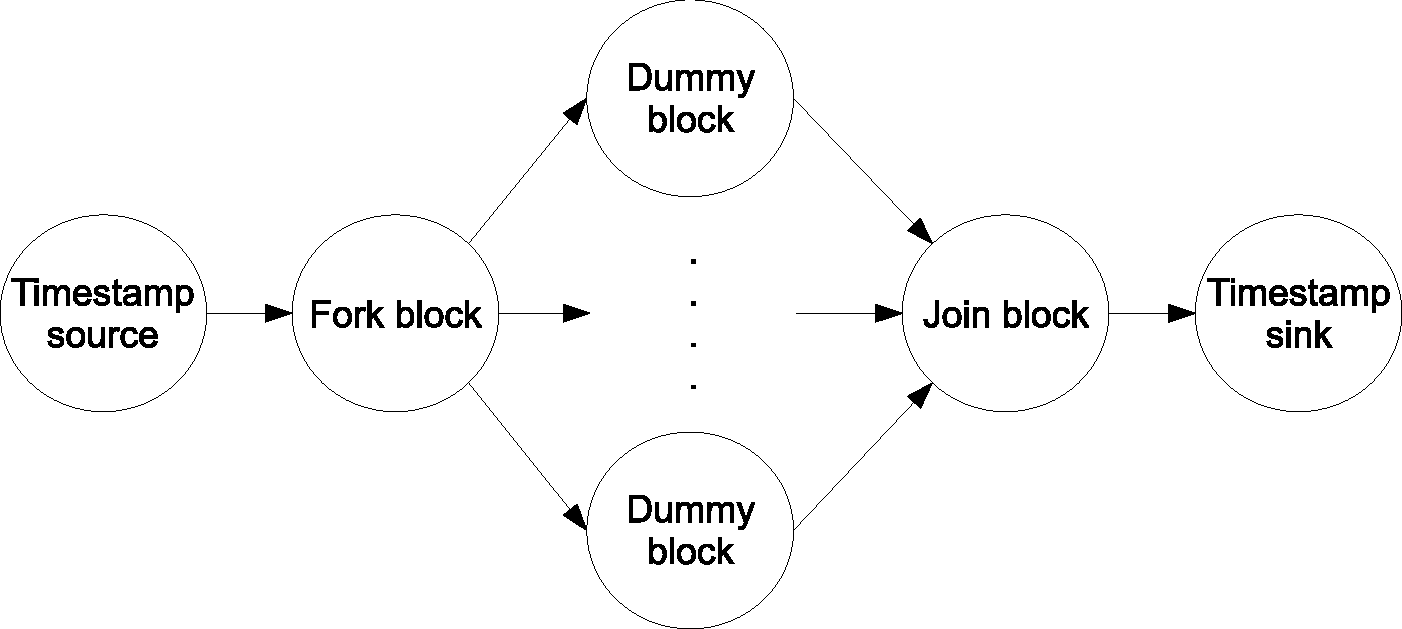
\includegraphics{fig/fig_arch_test_par}}}
  \newpage
  \subfloat[]{\label{fig_arch_test_par2}\scalebox{0.3}{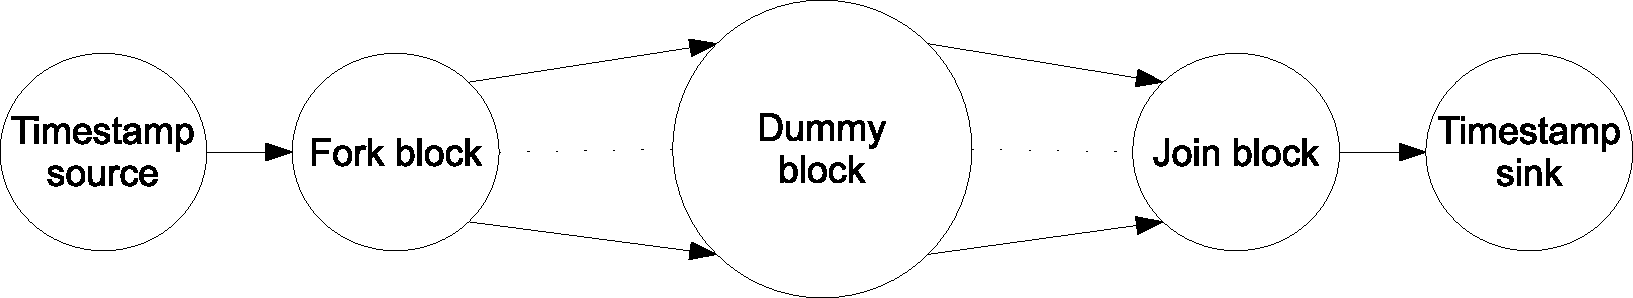
\includegraphics{fig/fig_arch_test_par2}}}
  \caption{SDRs data flow structures used for the overhead evaluation in terms of the number of blocks in serial (a), the number of data flows in parallel (b), and the number of inputs/outputs (c)}
  \label{fig_arch_test_all}
\end{figure}

These structures are composed by three kinds of blocks. The \emph{Timestamp source} block generates samples which consist of ti\-me\-stamps that represent the time when the sample was generated. The \emph{dummy blocks} are empty blocks that just propagate their inputs to their outputs. After being generated, the samples will go through the \emph{dummy block} chain. When a sample arrives at the \emph{Timestamp sink} block, the ti\-me\-stamp is compared with the current time, obtaining the time the sample took to go through the \emph{dummy block} chain. Since the \emph{dummy blocks} are empty, this resulting time represents only the overhead imposed by the architecture on the data flow. There is also the \emph{Fork block} and \emph{Join block} which are used to fork and join the data flows, respectively.

\subsection{System Implementation and Configuration}

To evaluate these three structures, we have implemented \hyra on the Xilinx's ML403 Embedded Platform~\cite{ML403}. The ML403 features a Virtex-4 FPGA with an embedded PowerPC 405 microprocessor. In order to use the same hardware configuration, we have synthesized the hardware with all of the necessary blocks for all experiments. Table \ref{table_ml403_sdr_arch_params} shows the parameters used in the experiment's setup. The $\alpha$ factor was fixed to $1$ in order to provide an evaluation considering low jitter requirements. The last four parameters are related to the configuration of the interconnect structure in hardware.

\begin{table}
%
\footnotesize
%
\begin{minipage}[c]{0.5\linewidth}
\centering
\caption{Configuration parameters used on the experiments}
\label{table_ml403_sdr_arch_params}

\begin{tabular}{ll}
\hline\noalign{\smallskip}
Parameter & Value \\
\noalign{\smallskip}
\hline
\noalign{\smallskip}
Synthesis tool & ISE/EDK 10.1 \\
Compiler & GCC 4.0.2 \\
FPGA clock & 100 MHz \\
Microprocessor clock & 100 MHz \\
$\alpha$ & 1 \\
Num. of input ports & 32 \\
Num. of output ports & 32 \\
HW FIFO size & 8 bits wide with 16 elements \\
Num. of FIFOs & 64 \\
\hline
\end{tabular}
\end{minipage}
%
%
\begin{minipage}[c]{0.5\linewidth}
\centering
\caption{Amount of HW resources used by the synthesized structures}
\label{table_ml403_sdr_arch_synt}
%Should regenerate the hardware with the new structure to obtain more reliable results

\begin{tabular}{llll}
\hline\noalign{\smallskip}
Resource & Our IPs & EDK IPs & Full System \\
\noalign{\smallskip}
\hline
\noalign{\smallskip}
4-input LUTs & 37\% & 35\% & 72\% \\
Slice Flip Flops & 67\% & 31\% & 98\% \\
Occupied Slices & 70\% & 55\% & 99\% \\
RAM blocks & 0\% & 63\% & 63\% \\
Max. frequency & 167 MHz & 109 MHz & 107 MHz \\
\hline
\end{tabular}

\end{minipage}
%
\normalsize
%
\end{table}

%juntei com table_ml403_sdr_arch_synt lado a lado
%\tab{table_ml403_sdr_arch_params}{Configuration parameters used on the experiments}

Table \ref{table_ml403_sdr_arch_synt} shows the resource consumption of the generated hardware. Separate results are shown for \hyra's structures along with the HW dummy blocks, and for the system IPs generated by EDK (internal memory, memory controller, interruption controller, UART, etc). Due to the lack of memory blocks available on the device, we chose to implement the FIFOs using the SRL16 capabilities to convert a 4-input LUT into a 16-bit shift register. This feature not only allows us to save memory blocks, but also yields high performance and low cost FIFO implementation~\cite{chapman08}. 

Our architecture alone uses about 65\% of the available device resources. This apparently high resource usage is due to the very limited amount of logic available on the device used. When compared to other system IPs, we can see that \hyra uses slightly more resources then a complete set of basic IO and memory peripherals. Also, if we consider that a mid-end Xilinx Spartan-6~\cite{XILINX_SPARTAN_6} FPGA has about 10 times more logic resources then the Virtex-4 device in the ML403 platform, our architecture imposes negligible area overhead in more recent devices.

%Additionally, the application along with the EPOS operating 
%system compiled for the PowerPC processor resulted in a memory footprint of 47632 bytes of code and 288 bytes of static data.

%juntei com table_ml403_sdr_arch_params lado a lado
%\tab{table_ml403_sdr_arch_synt}{Amount of HW resources used by the synthesized structures}


\subsection{Performance Overhead}

We have done tests to determine the performance overhead that we defined as the latency between the \emph{Timestamp source and sink} blocks in the three basic data flow structures. We have implemented each structure in hardware and software and executed tests with the number of dummy blocks ranging from 1 to 16. In each test $6\times10^7$ samples were generated and we obtained the average value of the latencies of each sample and the standard deviation. We used the standard deviation to obtain the coefficient of variation which yields normalized values for the overhead variation among the various configurations. A sampling rate of $1\times10^6$ samples/second was used in the tests with blocks in hardware. For the tests with blocks in software we used a sampling rate of $1\times10^4$ due to the low speed of the PowerPC processor.

Figures \ref{fig_result_mean_ppc_hw} and \ref{fig_result_coef_ppc_hw} show the results. When using only software blocks, the overhead grows linearly in relation to the increase in the number of blocks and the number of inputs and outputs for all structures. The coefficient of variation remained low in all configurations, and the lowest values for the multiple input/output dummy block configurations were due to the constant number of threads in the system. When using only HW blocks, the latency was about four orders of magnitude lower than when using software blocks and, as expected, except for the serial block configuration, the latency remained constant regardless the size of the structure, due to the full parallelism that can be explored in this kind of architecture. There is also a null coefficient of variation in the hardware operations.

%\fig{0.4}{fig_result_mean_ppc_hw}{Average latency for blocks in serial, in parallel and with multiple input/output}

%\fig{0.4}{fig_result_coef_ppc_hw}{Coefficient of variation of the proposed architecture latency}

%\begin{figure}
%  \centering
%  \subfloat[Average latency]{\label{fig_result_mean_ppc_hw}\scalebox{0.4}{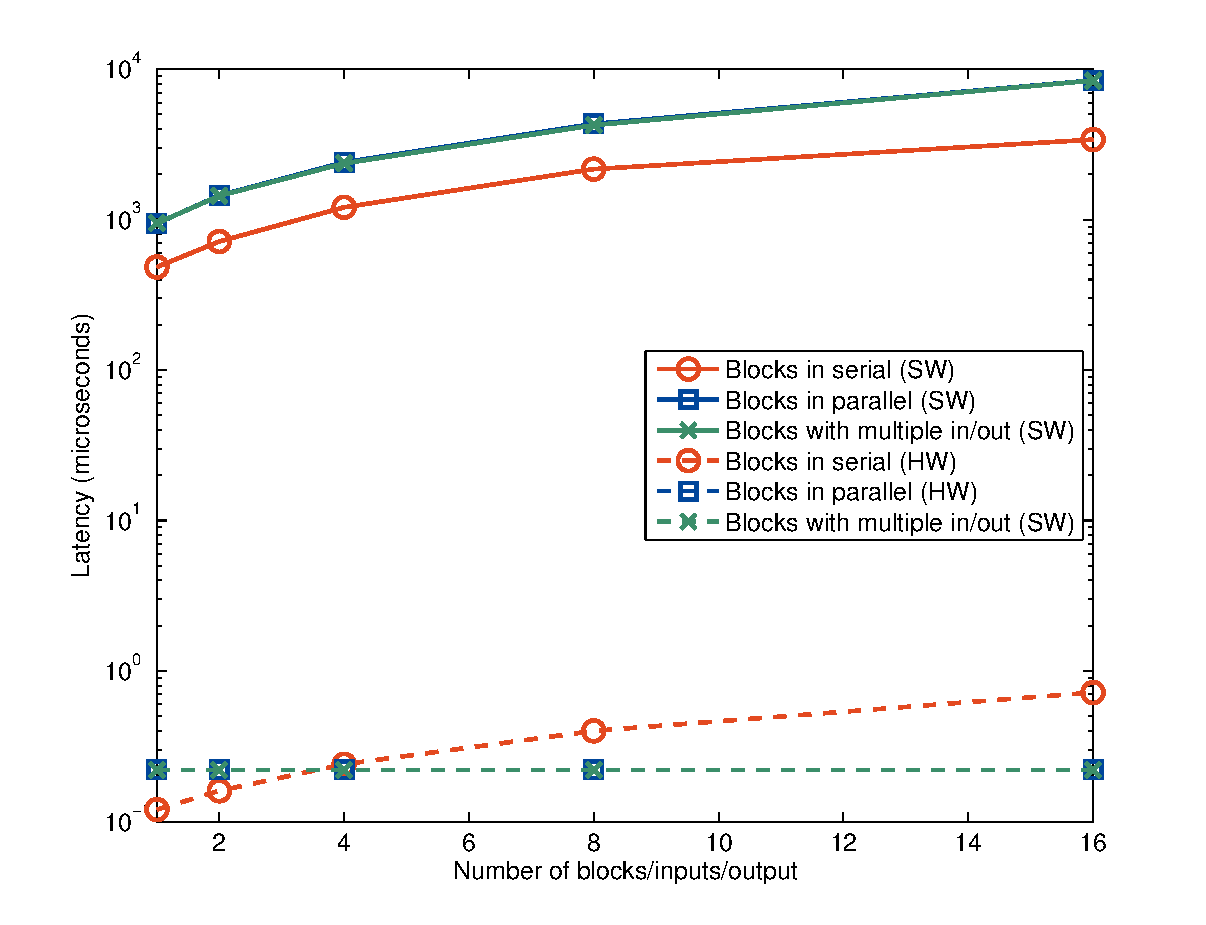
\includegraphics{fig/fig_result_mean_ppc_hw}}} \\
%  \subfloat[Coefficient of variation]{\label{fig_result_coef_ppc_hw}\scalebox{0.4}{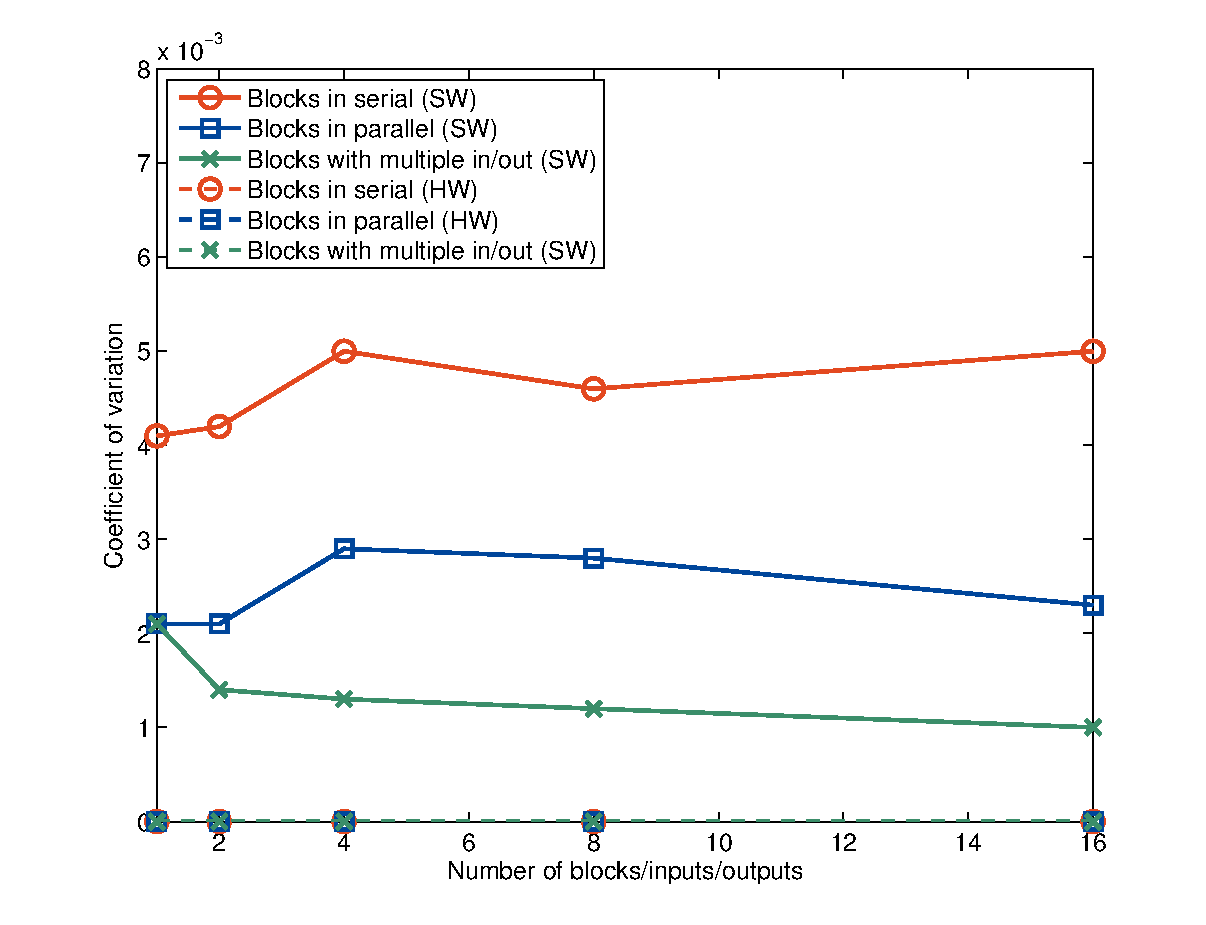
\includegraphics{fig/fig_result_coef_ppc_hw}}}
%  \caption{Latency for blocks in serial, in parallel, and with multiple input/output}
%  \label{fig_result_ppc_hw}
%\end{figure}


\begin{figure}[ht]
  \begin{minipage}[htbp]{0.5\linewidth}
    \centering
    \scalebox{0.4}{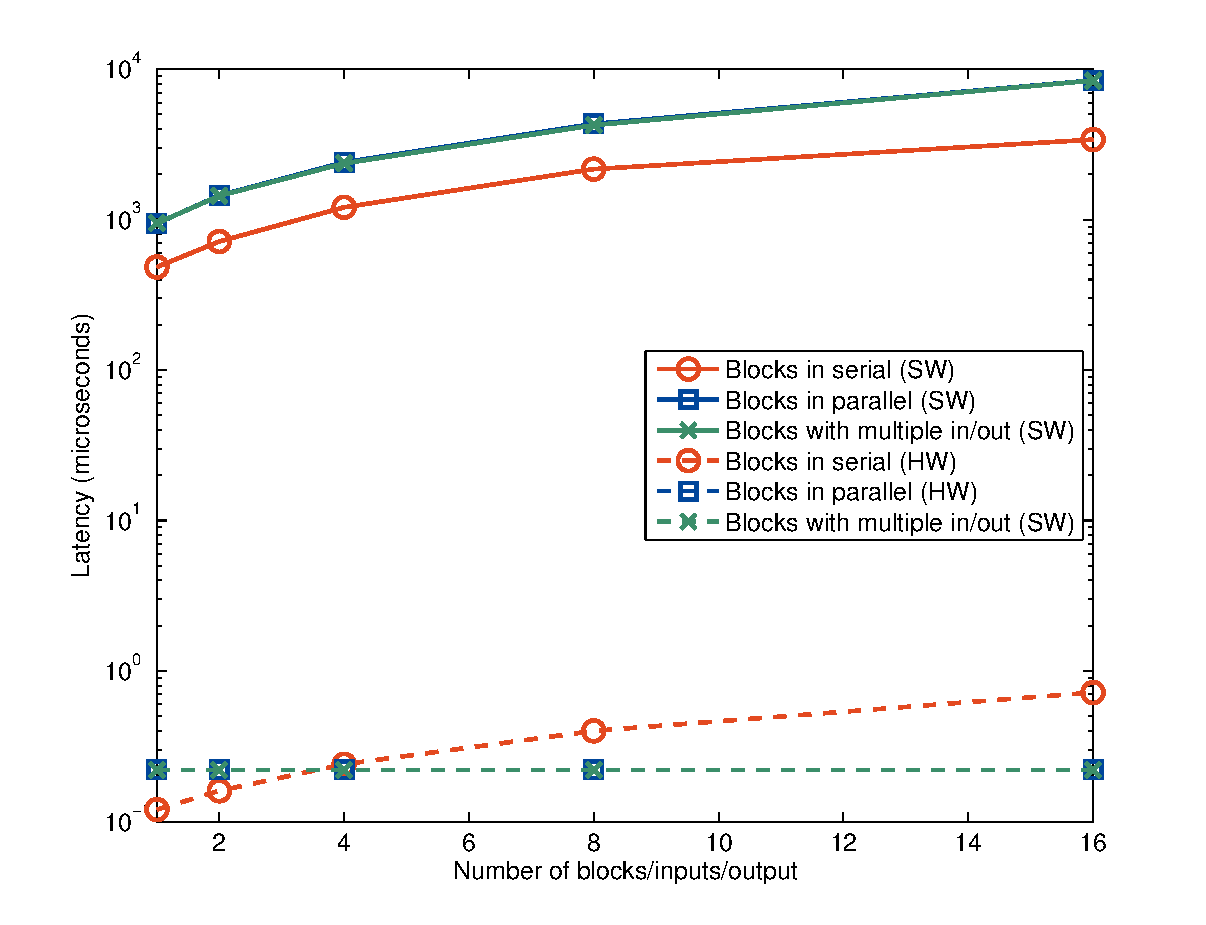
\includegraphics{fig/fig_result_mean_ppc_hw}}
    \caption{Average latency for blocks in serial, in parallel and with multiple input/output}
    \label{fig_result_mean_ppc_hw}
  \end{minipage}
  \hspace{0.5cm}
  \begin{minipage}[htbp]{0.5\linewidth}
    \centering
    \scalebox{0.4}{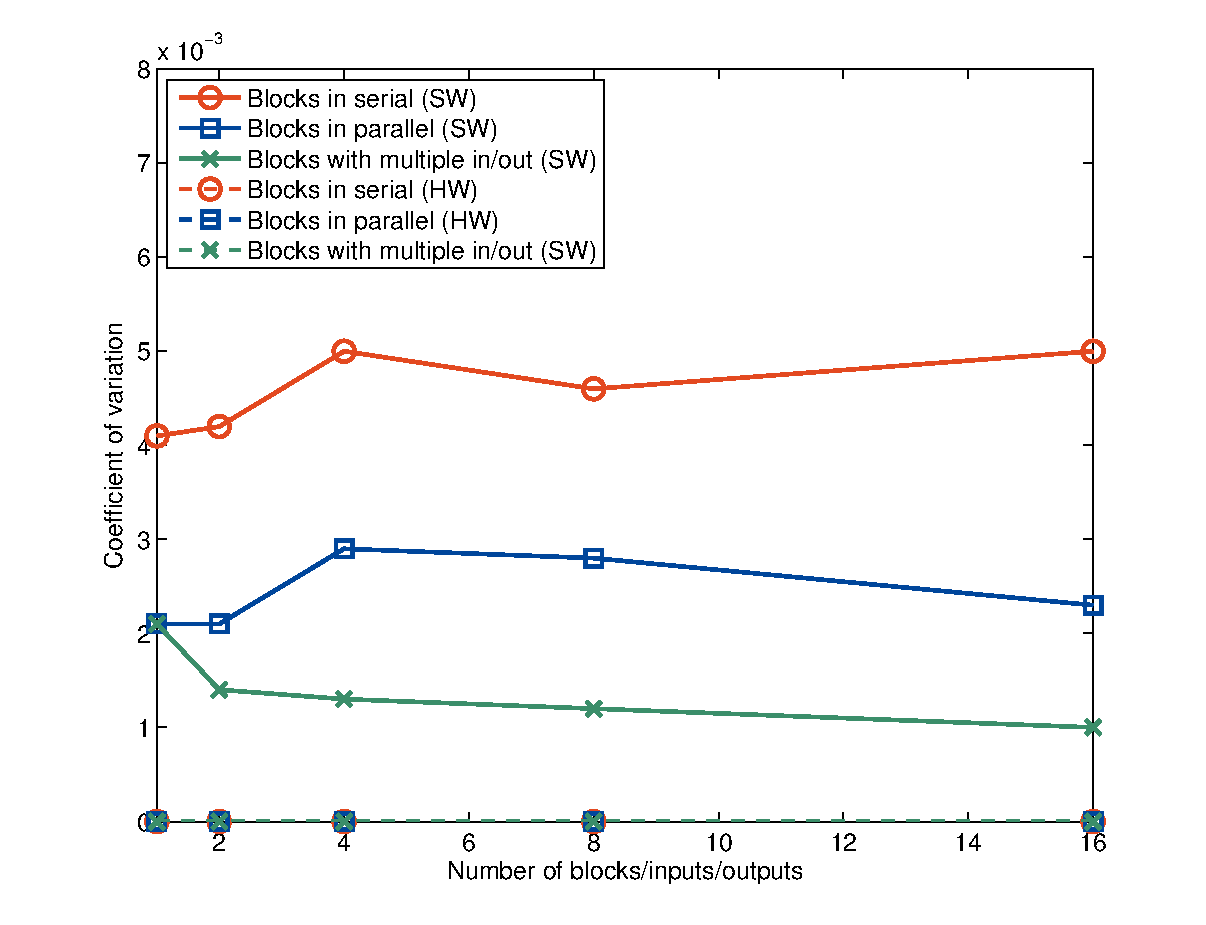
\includegraphics{fig/fig_result_coef_ppc_hw}}
    \caption{Coefficient of variation of the proposed architecture latency}
    \label{fig_result_coef_ppc_hw}
  \end{minipage}
\end{figure}


To evaluate de latency in the communication between components implemented in HW and components implemented in SW, we used the data flow shown in figure \ref{fig_result_sw_hw_data_flow} which cover operations on both \emph{SW-HW FIFOs} and \emph{HW-SW FIFOs}. We evaluated both source/sink components in SW and HW. Figure \ref{fig_result_sw_hw} shows the results of the same tests described previously executed on this two structures, and compares with the results obtained for SW and HW only components. Both interleaved data flows yielded similar results. Data flow (a) have more SW blocks then (b), thus showing a higher SW management overhead. However, both have two \emph{SW-HW FIFOs} and two \emph{HW-SW FIFOs} connecting the blocks, which shows that the read/write operations in the channels represents the most significant overhead.


\fig{0.4}{fig_result_sw_hw_data_flow}{Serial data flows with interleaved SW and HW blocks}

\fig{0.4}{fig_result_sw_hw}{Average latencies on the serial data flow with interleaved SW and HW blocks}

We also compared the overhead of our architecture to GNU Radio. For this comparison, we replicated the same tests described previously using GNU Radio running over a Linux operating system in a PC. Our architecture and EPOS were compiled for the IA32 architecture only with software blocks support, and evaluated in the same system. For the GNU Radio experiment, we used GNU Radio 3.2.2 running on a Linux kernel 2.6.28 and, in order to avoid interference from other Linux processes, the GNU Radio application was executed using the \emph{enable real-time scheduling} feature, which gives the highest priority to the GNU Radio process. The result for the serial blocks data flow structure shown in figure \ref{fig_result_mean_ia32_gnu} demonstrates that our architecture performance surpasses GNU Radio between 2 and 4 times, and this difference increases as the number of blocks in the processing chain increases. Figure \ref{fig_result_coef_ia32_gnu} also shows that we are able to achieve smaller latency variations as well.

%\fig[h]{0.4}{fig_result_mean_ia32_gnu}{Average latency of the proposed architecture VS GNU Radio on the serial blocks data flow structure}

%\fig[h]{0.4}{fig_result_coef_ia32_gnu}{Coefficient of variation of the proposed architecture latency VS GNU Radio on the serial blocks data flow structure}

%\begin{figure}[t]
%  \centering
%  \subfloat[Average latency]{\label{fig_result_mean_ia32_gnu}\scalebox{0.4}{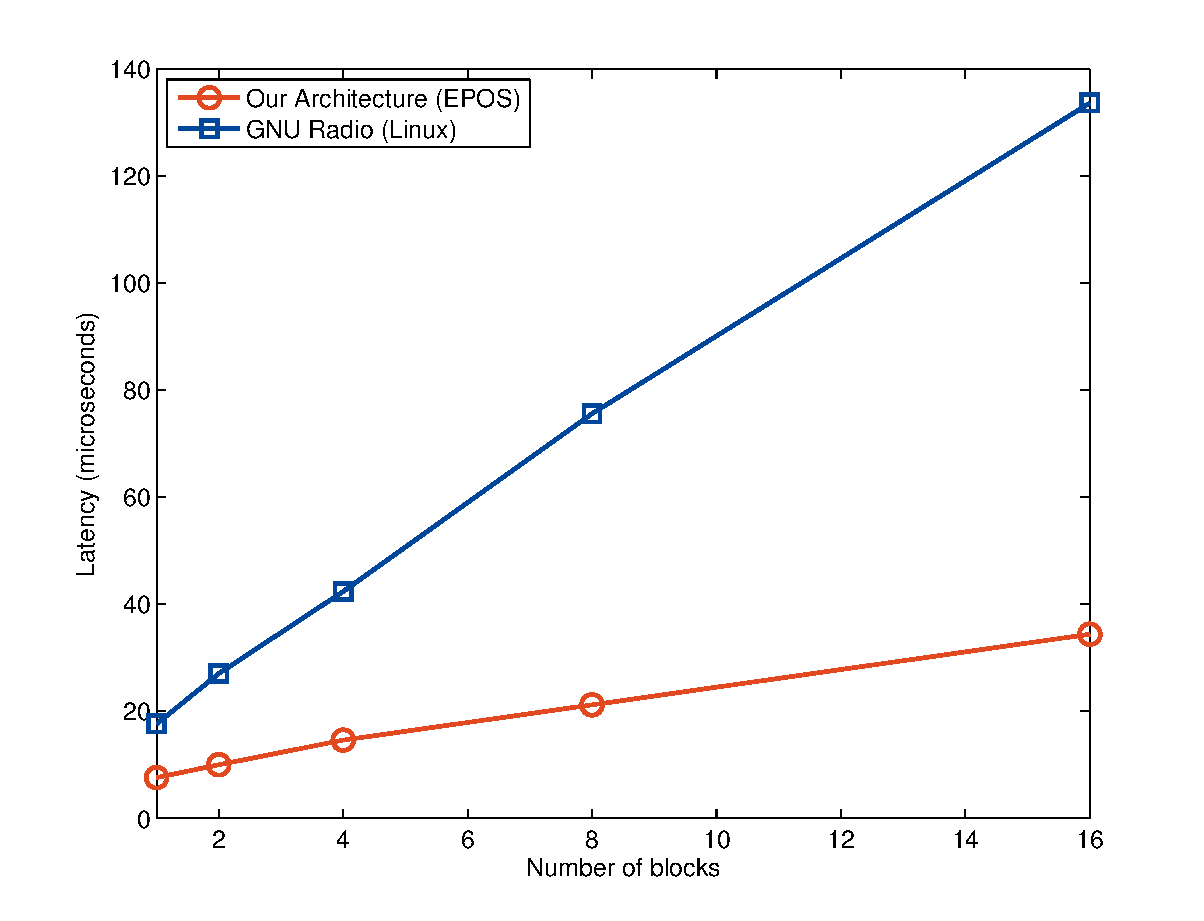
\includegraphics{fig/fig_result_mean_ia32_gnu}}} \\               
%  \subfloat[Coefficient of variation]{\label{fig_result_coef_ia32_gnu}\scalebox{0.4}{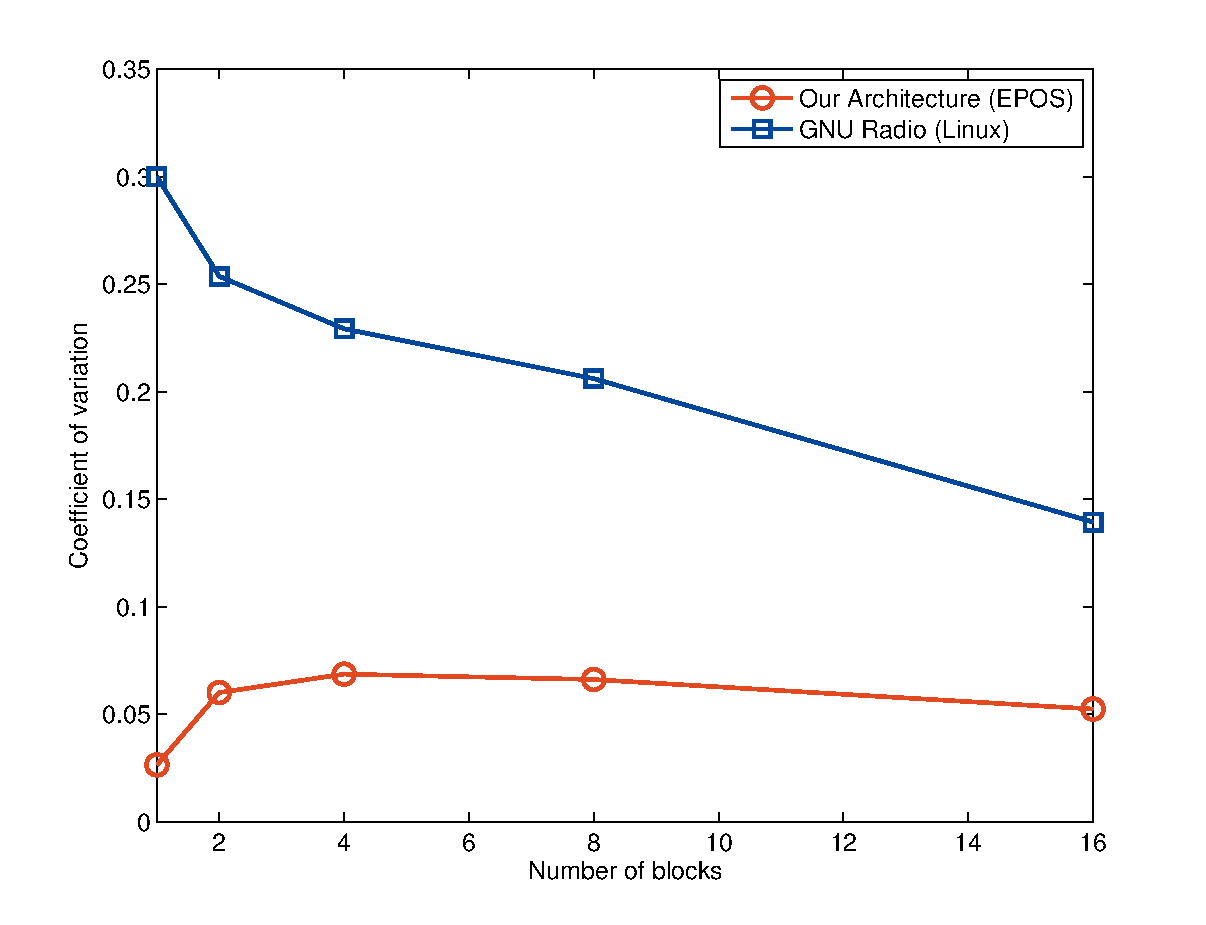
\includegraphics{fig/fig_result_coef_ia32_gnu}}}
%  \caption{Latency of the proposed architecture VS GNU Radio on the serial blocks data flow structure}
%  \label{fig_result_ia32_gnu}
%\end{figure}

\begin{figure}[ht]
  \begin{minipage}[htbp]{0.5\linewidth}
    \centering
    \scalebox{0.4}{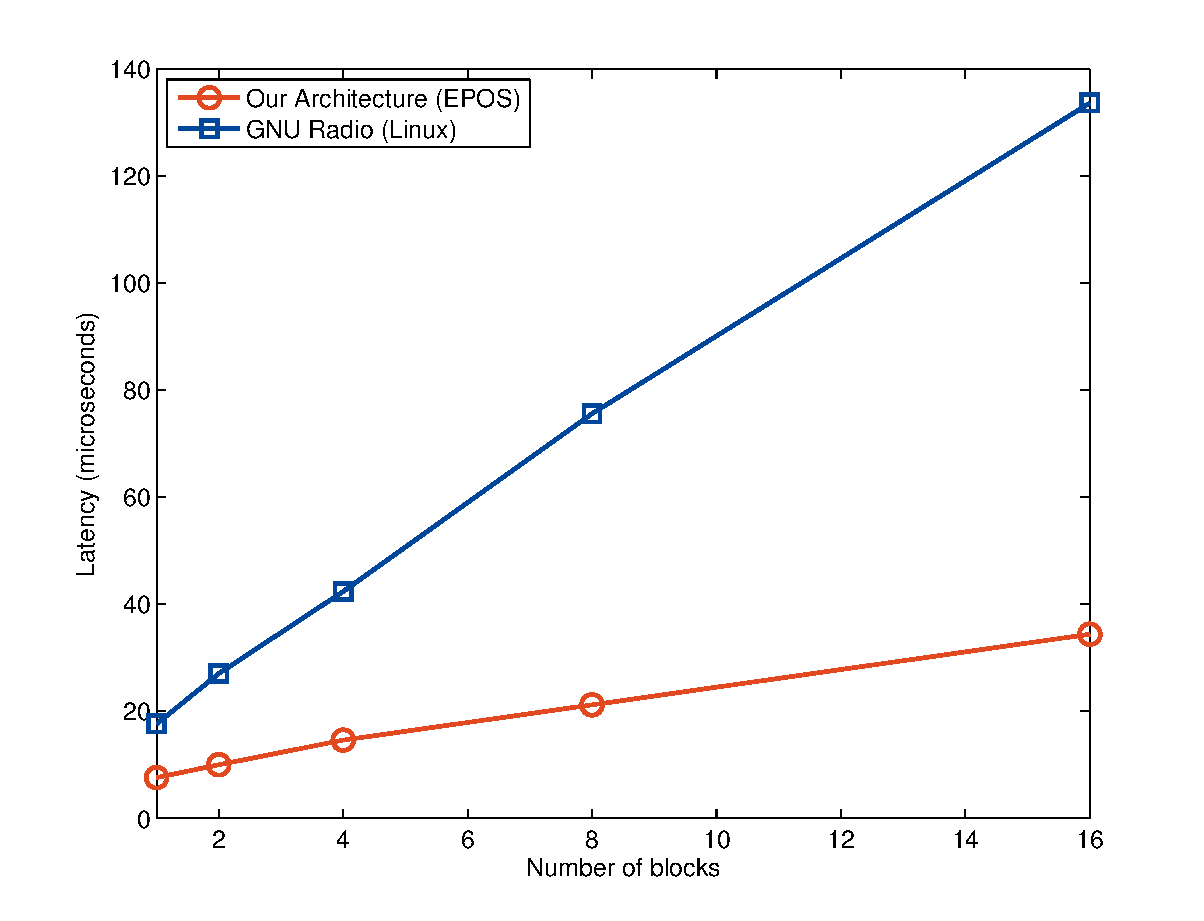
\includegraphics{fig/fig_result_mean_ia32_gnu}}
    \caption{Average latency of the proposed architecture VS GNU Radio on the serial blocks data flow structure}
    \label{fig_result_mean_ia32_gnu}
  \end{minipage}
  \hspace{0.5cm}
  \begin{minipage}[htbp]{0.5\linewidth}
    \centering
    \scalebox{0.4}{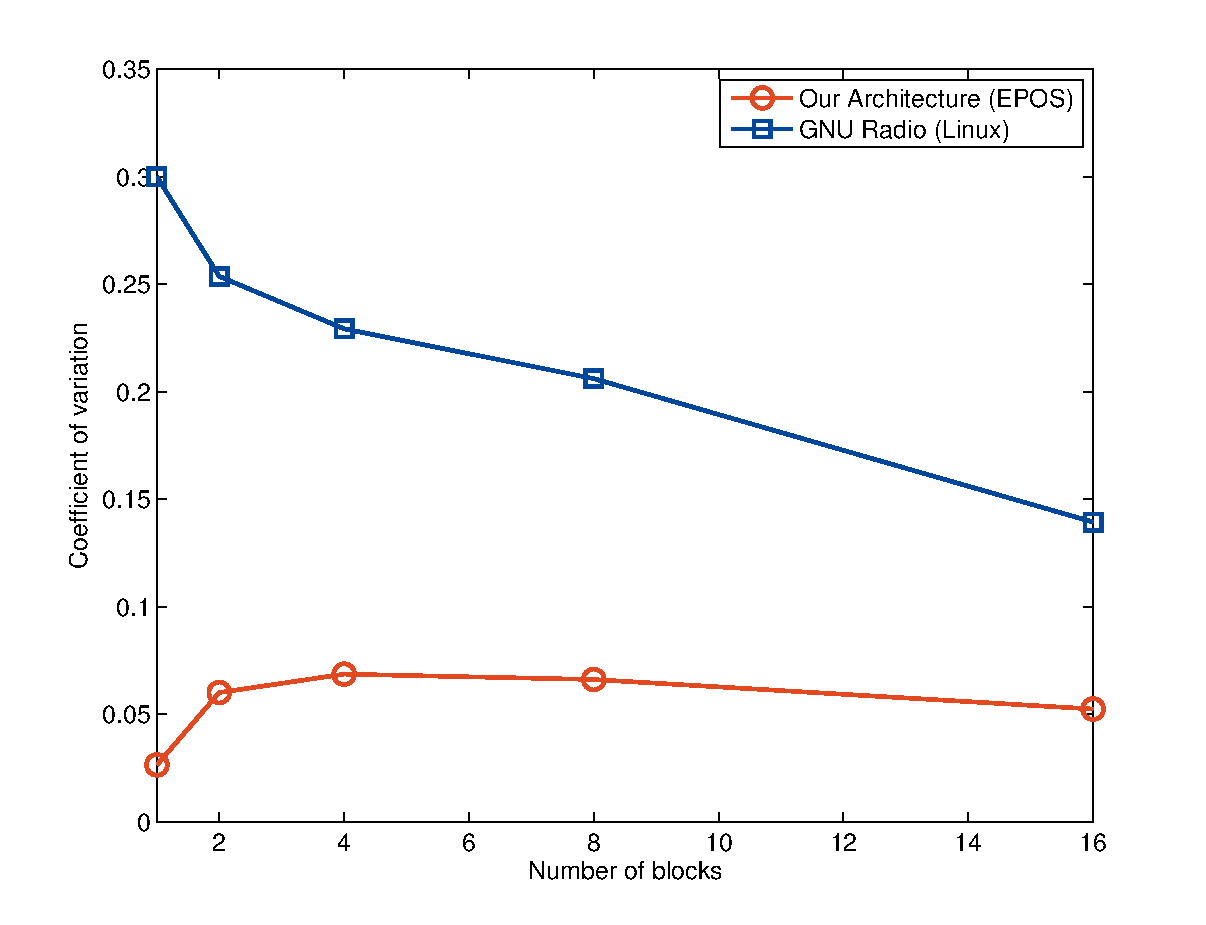
\includegraphics{fig/fig_result_coef_ia32_gnu}}
    \caption{Coefficient of variation of the proposed architecture latency VS GNU Radio on the serial blocks data flow structure}
    \label{fig_result_coef_ia32_gnu}
  \end{minipage}
\end{figure}


\subsection{Discussion}

The results show that our architecture yields superior performance than an equivalent, in terms of abstraction level, commonly used architecture. Only software components were used in this comparison, if a hardware device was used to generate the timestamps, GNU Radio would suffer an additional disadvantage. In GNU Radio, the use of any hardware device to obtain or sink data from/to the environment requires Linux drivers whose performance is mostly limited by the kernel's abstraction layer. A previous work~\cite{nychis09} shows that, due to the Linux kernel overhead, the standard deviation of the time a sample takes to get to the processing chain after being generated in the RF Front-end is higher than the average time. This problem does not appear in EPOS mainly for two reasons. First, EPOS is application specific: only the components required by the application are included in the system, and all of OS resources are dedicated towards a single application. Second, the metaprogrammed hardware mediators are dissolved within the application when the system is compiled, which leads to higher performance. Also, the virtually null variation obtained when hardware blocks are used in a dedicated platform (ML403) is especially important when implementing time-strict protocols, like TDMA based protocols.

However, even with known latency problem, the GNU Radio is widely used and several protocols have been succesfully implemented using it. The results have shown that with our architecture we were able to bring similar functionality with superior performance to the embedded system domain, which leads to the conclusion that our architecture is suitable for the implementation of high-end protocols in embedded systems.

%%%%%%%%%%%%%%%%%%%%%%%%%%%%%%%%%%%%%%%%%%%%%%%%%%%%%%%%%%%%%%%%%%%%%%%%%%%%%%
\section{Conclusion}
\label{CONCLUSION}

In this paper we have introduced \hyra, an \emph{Hybrid Radio
 Architecture} that explores the \emph{Hybrid Component} concept within
ADESD to enable the implementation of SDRs as direct mappings of
high-level SDF models. Each SDR functional block in the SDF model is
implemented as an hybrid component that can be subsequently plugged into
\hyra's framework. As hybrid components, \hyra\ SDR blocks can be
implemented as arbitrary combination of software and hardware on
FPGA-based platforms.  The programmable interconnect infrastructure in
\hyra's framework ensures transparency in this respect.  FIFO channels
can be fine tuned to fulfill the requirements of a given SDR protocol,
while the controller dynamically coordinates the flow of data between
components.

In comparison with other approaches, \hyra\ addresses the implementation
of SDRs in the context of embedded systems from a higher level of
abstraction. Yet the evaluation results presented in this paper confirm
that the overhead caused by the proposed architecture in terms of
latency and general resource consumption is much smaller than that of
GNU Radio, a widely accepted architecture. Furthermore, our experiments
demonstrated that \hyra\ can be implemented on reconfigurable hardware
platform with minimal additional resources. In combination, this factors
confirm that our architecture meet the requirements for the
implementation of high-end protocols in embedded systems.

\bibliographystyle{IEEEtran}
\bibliography{sdr.bib}

\end{document}



